\chapter{Painted Easter Eggs}
\label{ch:eastereggs}
\index{Easter}

\marginnote{
    \textbf{Makes 48 painted eggs} \\
    Prep time: 10 minutes \\
    Cook time: 20 minutes \\
    \vspace*{\baselineskip}

    \textbf{Ingredients for cookies} \\
    48 eggs \\
    1 pack of Red Dye for Eggs, Rida \\
    1/2 cup vinegar \\
    Vegetable oil
}

Family member: Mom

\newthought{After every} Easter dinner we would all gather around the table to break the painted eggs. At the end, we would have egg shell on the entire table and our hands would be red! And every year, a different person would have the "strongest" egg!     The dye can be found at Greek bakeries such as at Afroditi or Serano Bakery in Laval. Mom found this method to yield the deepest red colored eggs.

\begin{enumerate}
    \item Boil the eggs and cool them.
    \item Empty the color in the pot filled with 1 liter of lukewarm water and the vinegar.
    \item Add enough eggs to be fully covered with the colored water. After 5 minutes, remove the eggs and place them on paper towel to drain the water.
    \item Wipe the eggs with some vegetable oil.
    \item Using the same colored water, do the same with the rest of the eggs. 
\end{enumerate}

\begin{marginfigure}[20pt]
  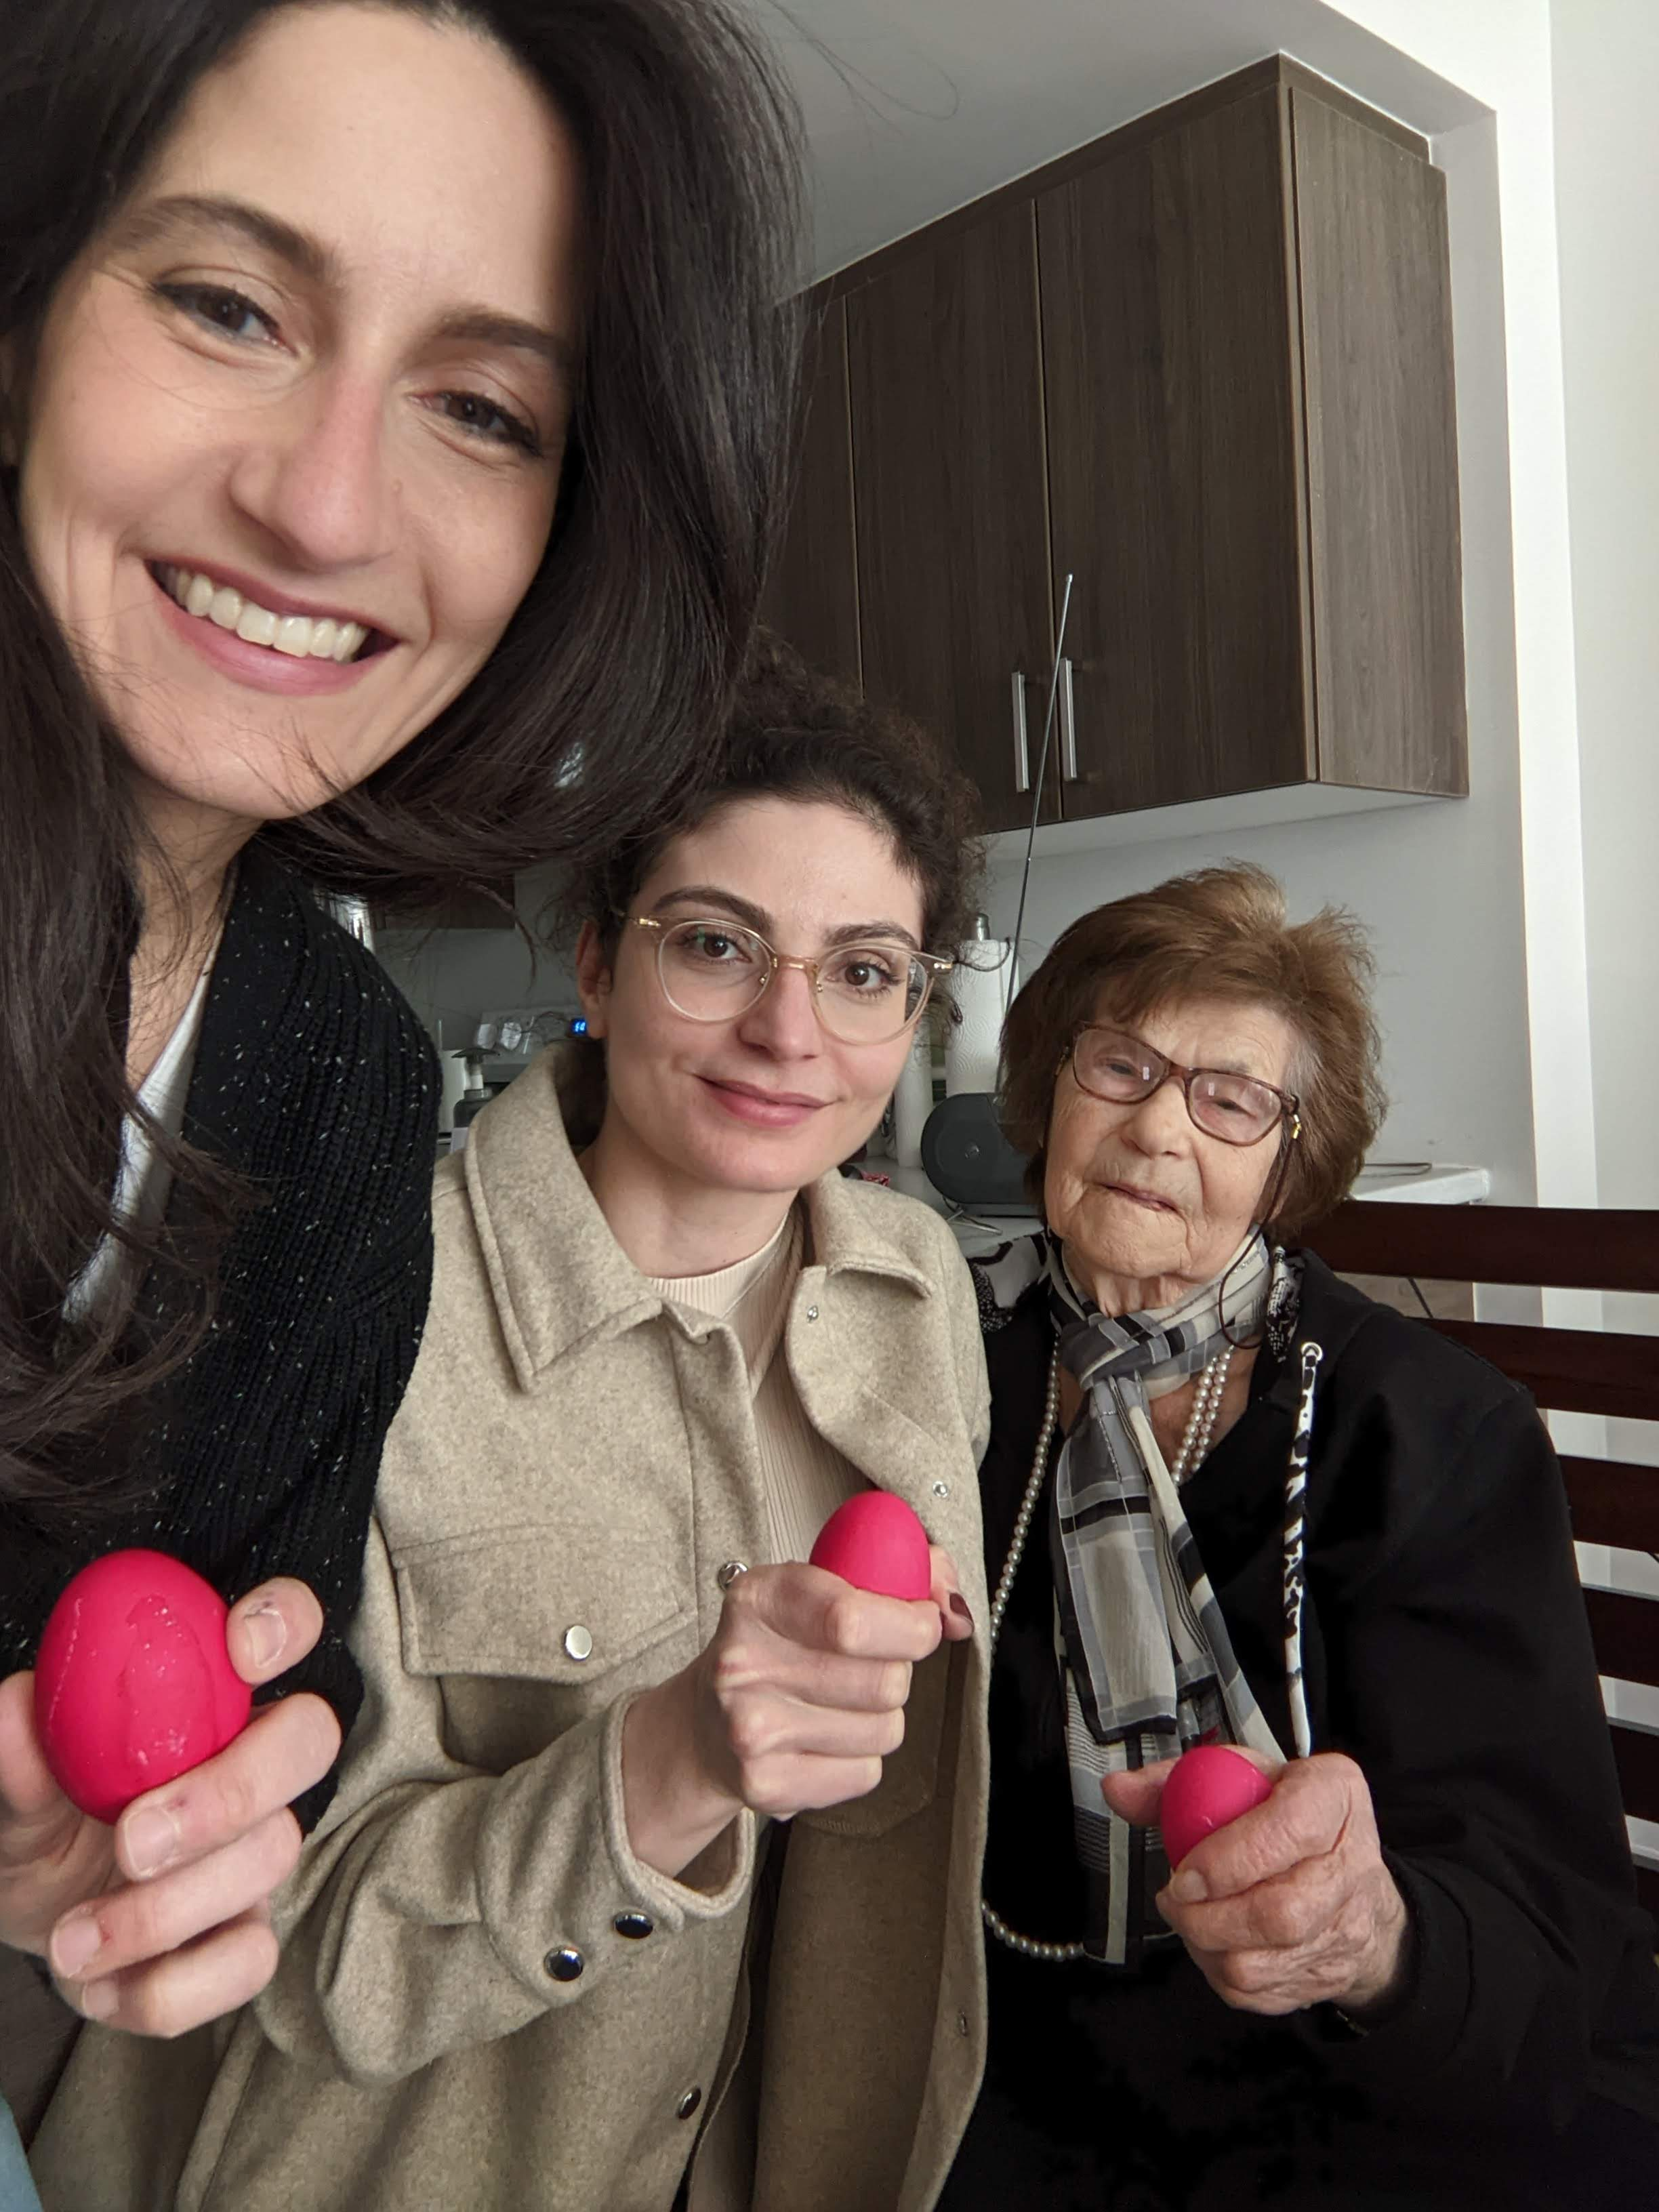
\includegraphics[width=60mm]{monanteras/images/Easter eggs with grandma.jpg}
  \caption{Easter with Grandma Eleni}
\end{marginfigure}

\begin{figure}
  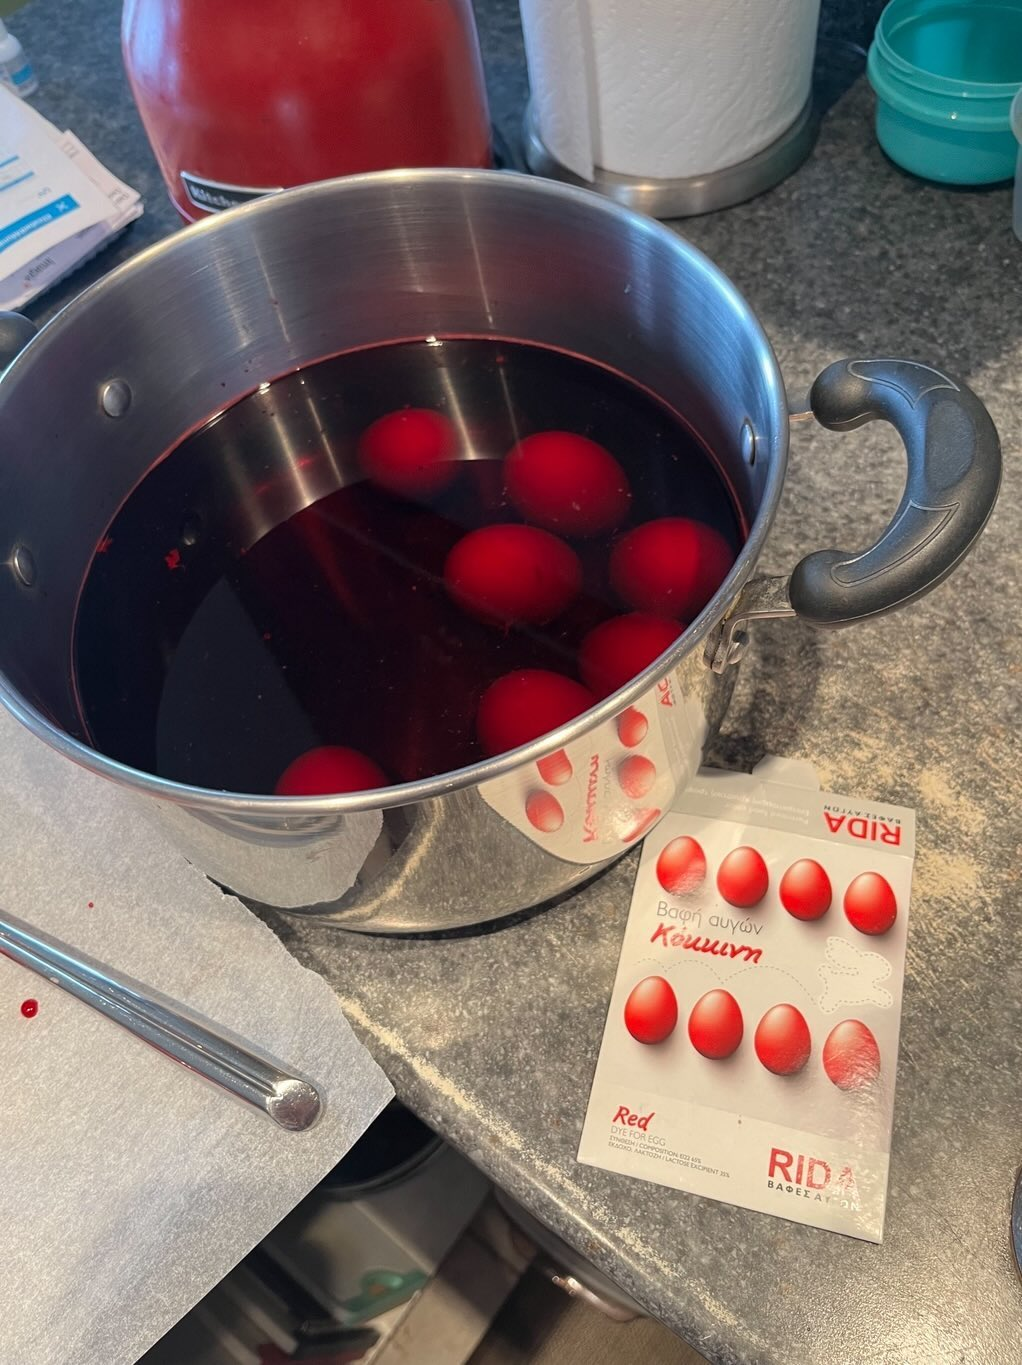
\includegraphics[width=60mm]{monanteras/images/Eggs 3.jpg}
\end{figure}
\begin{figure}
  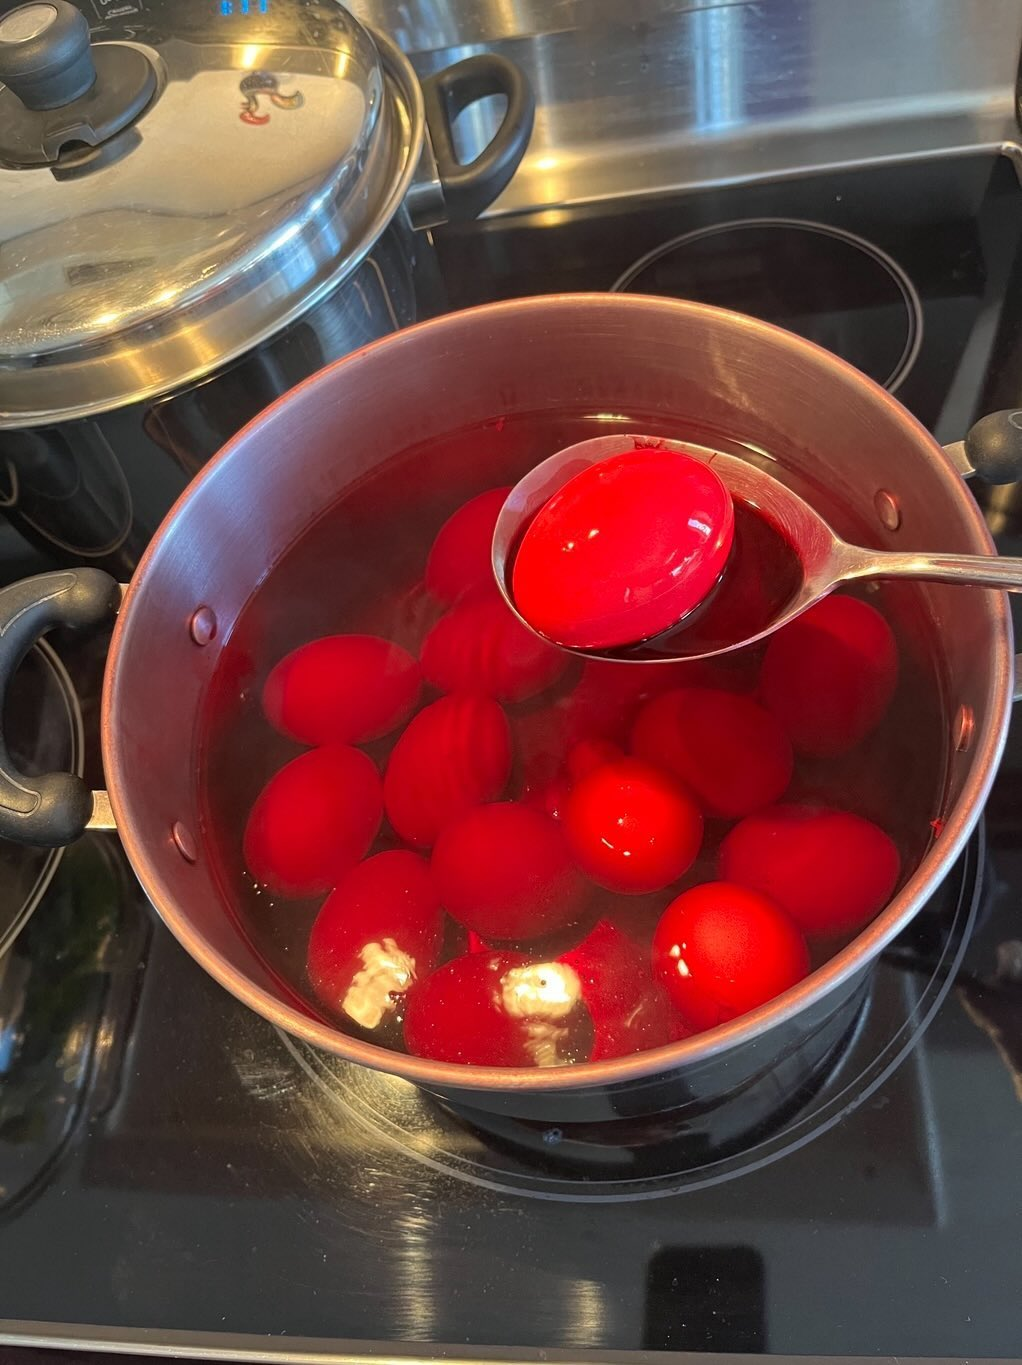
\includegraphics[width=60mm]{monanteras/images/Eggs 5.jpg}
\end{figure}
\begin{figure}
  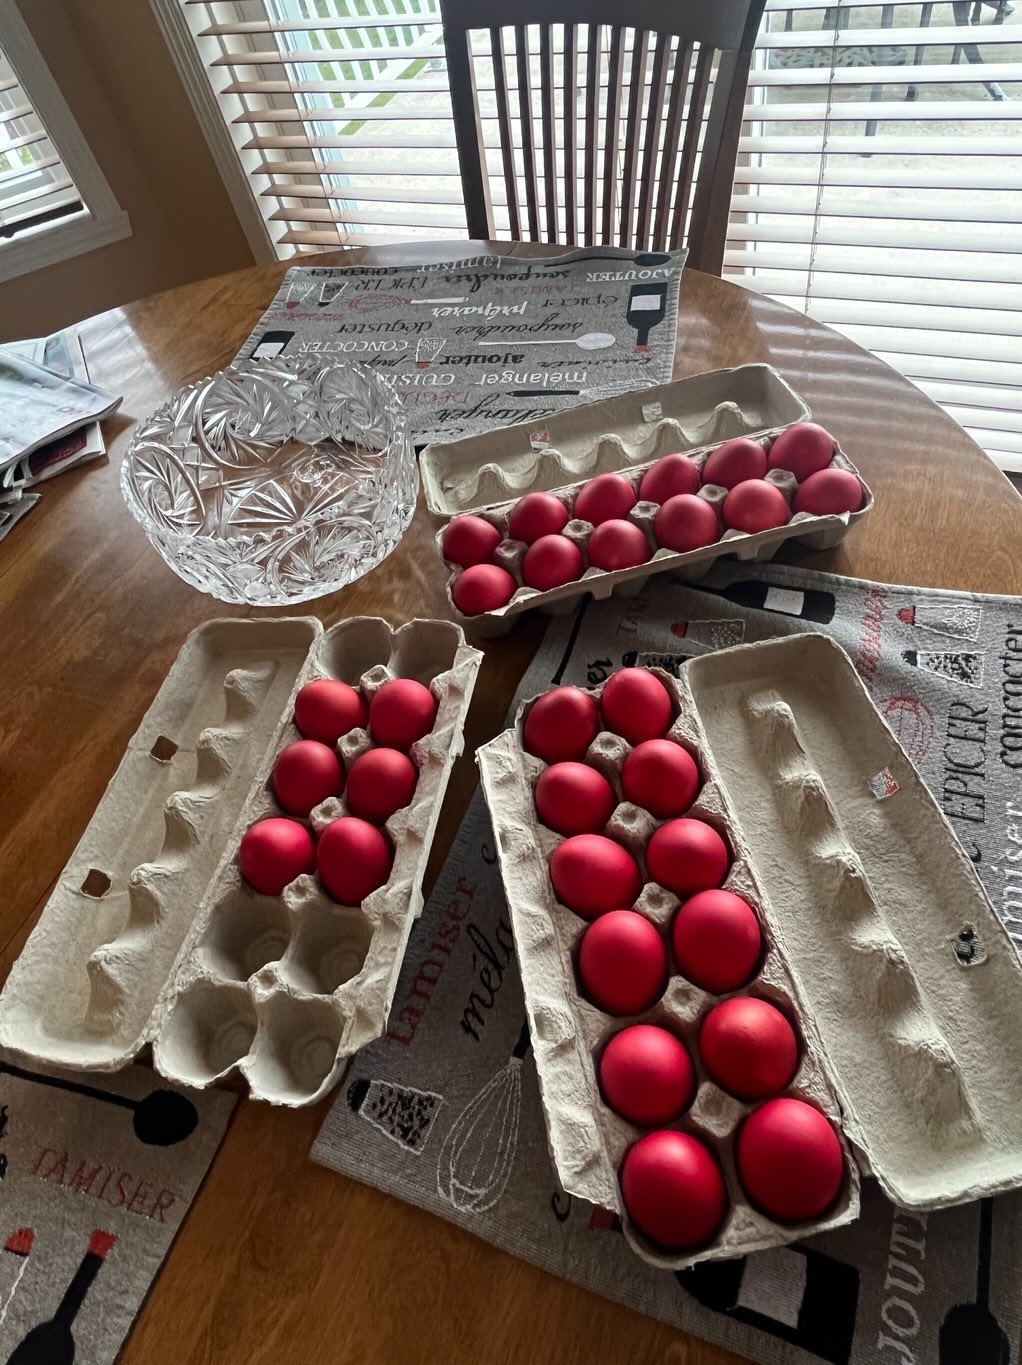
\includegraphics[width=60mm]{monanteras/images/Eggs 4.jpg}
\end{figure}
\begin{figure}
  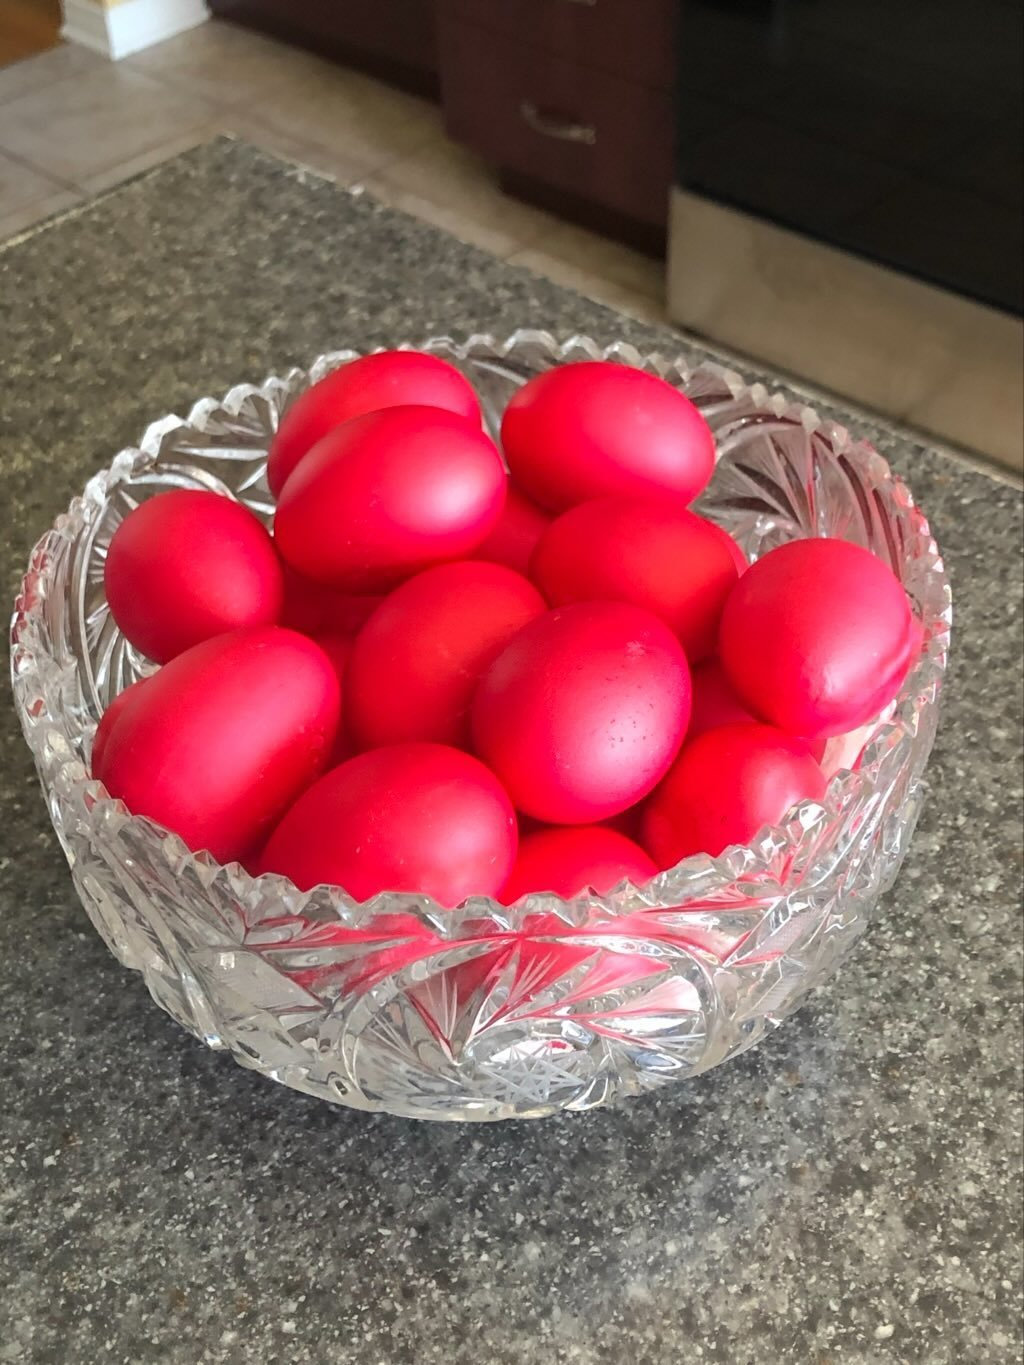
\includegraphics[width=60mm]{monanteras/images/Eggs 7.jpg}
\end{figure}
